\newpage
\section{Architettura}
\subsection{Informazioni Generali}
Il principio di progettazione che abbiamo addottato è il \termine{Common Closure Principale} per i seguenti motivi:
\begin{itemize}
\item Suddivizione più più logica dei vari package e classi.
\item Aumenta la manutenibilità del codice nel tempo.
\item 
\end{itemize}

\subsubsection{Suddivisione in package  di \termine{Monolith}}
\label{Monolith}
\begin{figure}[H]
	\centering
	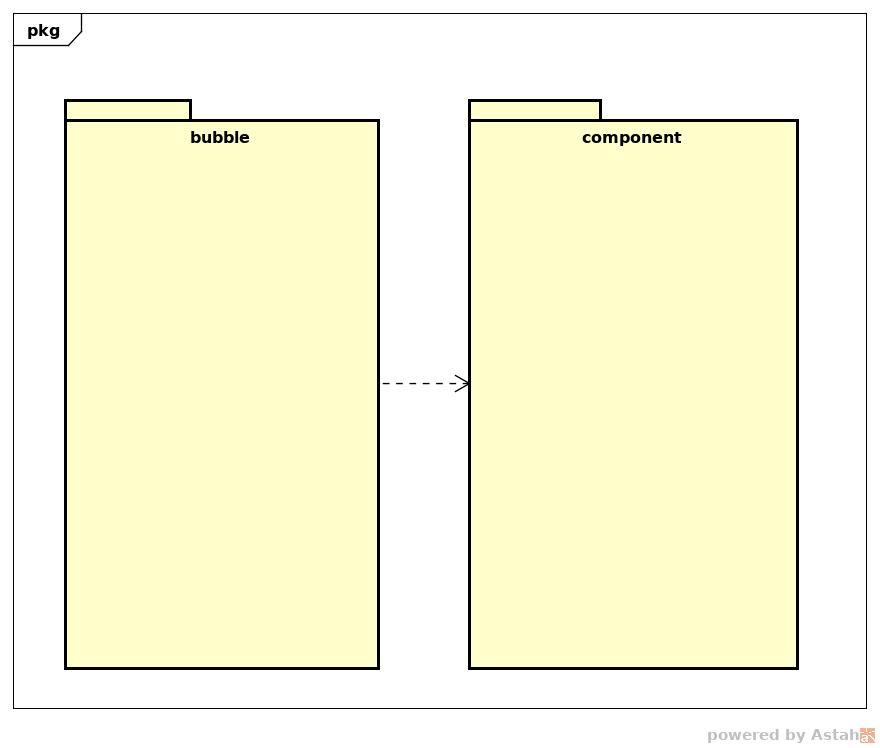
\includegraphics[scale=0.5]{Sezioni/imgPackage/Monolith.png}
	\caption{Monolith}
\end{figure}
\begin{itemize}
	\item{\textbf{Descrizione}}: architettura ad alto livello dell' \termine{SDK} \termine{Monolith}.
	\item{\textbf{Package e classi contenuti}}:
	\begin{itemize}
	\item{monolith::bubble}: package contenente tutti i package che compongono le bolle ed esso ha una dipendenza con il il package component.
	\item{monolith::component}: package contenente tutti i package dei componenti che compongono le bolle, ad esempio tutti i tipi di widget e layout.
	\end{itemize}
	
\end{itemize}


\subsubsection{Suddivisione in package  di Monolith::bubble}
\label{Monolith::bubble}
\begin{figure}[H]
	\centering
	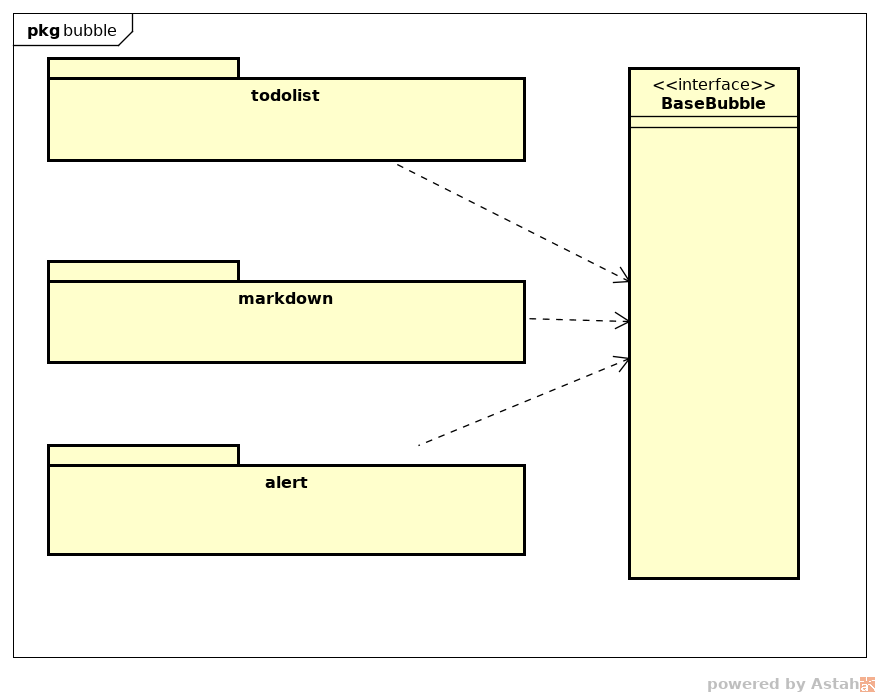
\includegraphics[scale=0.5]{Sezioni/imgPackage/bubble.png}
	\caption{Monolith::bubble}
\end{figure}
\begin{itemize}
	\item{\textbf{Descrizione}}: packege contenente tutti i tipi di bolle del \termine{SDK}.
	\item{\textbf{Package e classi contenuti}}:
	\begin{itemize}
	\item{monolith::bubble::todolist}: package contenente la classe per creare una bolla di tipo \termine{ToDoList}.
	\item{monolith::component::markdown}: package contenente la classe per creare una bolla di tipo \termine{markdown}.
	\item{monolith::component::alert}: package contenente la classe per creare una bolla di tipo \termine{alert}.
	
	\end{itemize}
	
\end{itemize}

\subsubsection{Suddivisione in package  di Monolith::bubble::todolist}
\label{Monolith::bubble::todolist}
\begin{figure}[H]
	\centering
	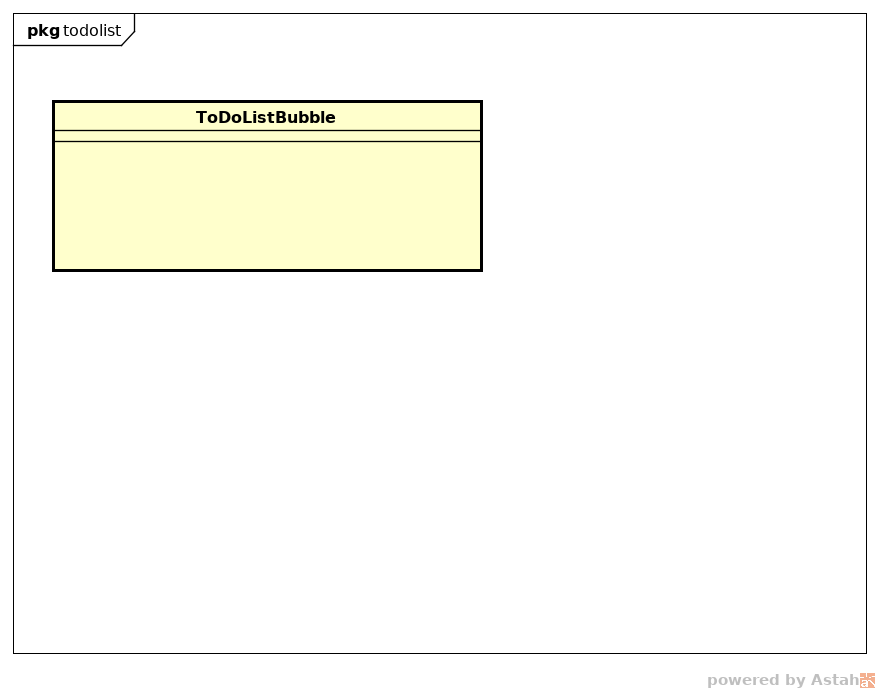
\includegraphics[scale=0.5]{Sezioni/imgPackage/bubble_todolist.png}
	\caption{Monolith::todolist}
\end{figure}
\begin{itemize}
	\item{\textbf{Descrizione}}: package contenente la classe per creare la bolla di tipo \termine{ToDoList}
	\item{\textbf{Classi contenuti}}:
	\begin{itemize}
	\item{monolith::bubble::ToDoListBubble}: classe per creare la bolla di tipo \termine{ToDoList}.
	\end{itemize}
\end{itemize}
	
\subsubsection{Suddivisione in package  di Monolith::bubble::markdown}
\label{Monolith::bubble::markdown}
\begin{figure}[H]
	\centering
	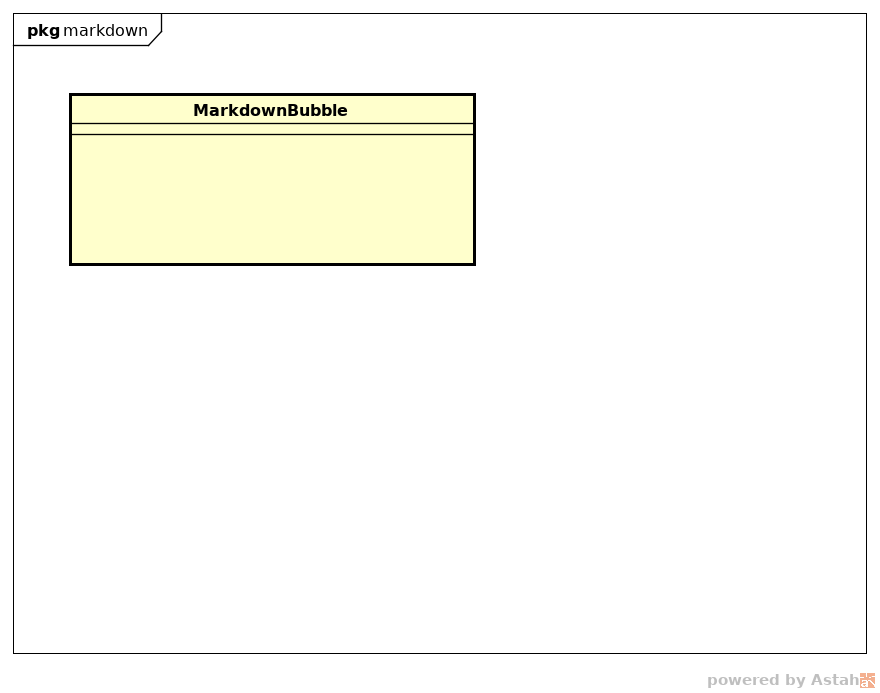
\includegraphics[scale=0.5]{Sezioni/imgPackage/bubble_markdown.png}
	\caption{Monolith::markdown}
\end{figure}
\begin{itemize}
	\item{\textbf{Descrizione}}: package contenente la classe per creare la bolla di tipo \termine{Markdown}
	\item{\textbf{Classi contenuti}}:
	\begin{itemize}
	\item{monolith::bubble::MarkDownBubble}: classe per creare la bolla di tipo \termine{MarkDown}.
	\end{itemize}
\end{itemize}

	\subsubsection{Suddivisione in package  di Monolith::bubble::alert}
\label{Monolith::bubble::alert}
\begin{figure}[H]
	\centering
	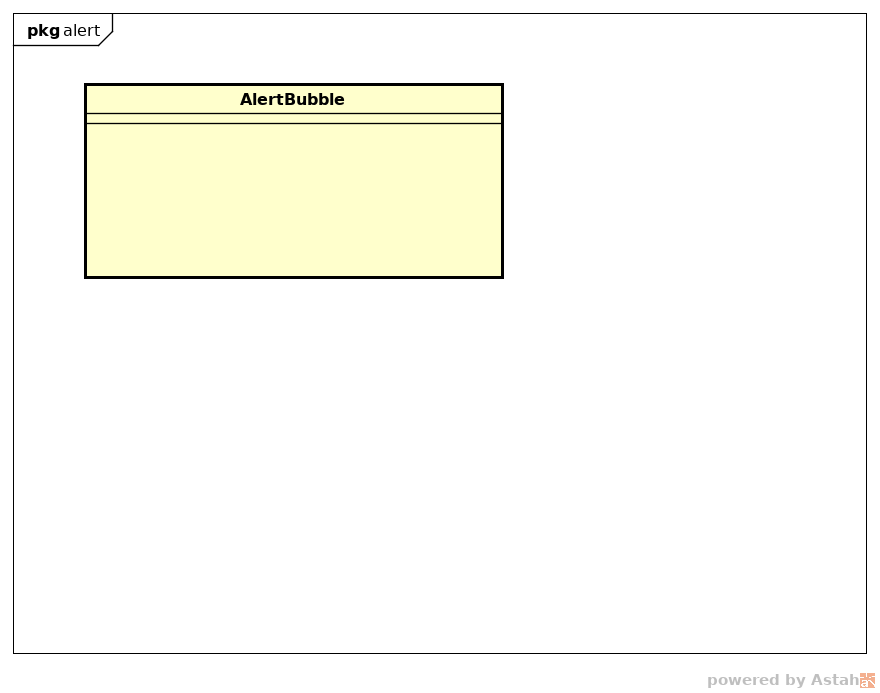
\includegraphics[scale=0.5]{Sezioni/imgPackage/bubble_alert.png}
	\caption{Monolith::bubble::alert}
\end{figure}
\begin{itemize}
	\item{\textbf{Descrizione}}: package contenente la classe per creare la bolla di tipo \termine{Alert}
	\item{\textbf{Package e classi contenuti}}:
	\begin{itemize}
	\item{monolith::bubble::AlertBubble}: classe per creare la bolla di tipo \termine{Alert}.
	\end{itemize}
\end{itemize}



\subsubsection{Suddivisione in package  di Monolith::component}
\label{Monolith::component}
\begin{figure}[H]
	\centering
	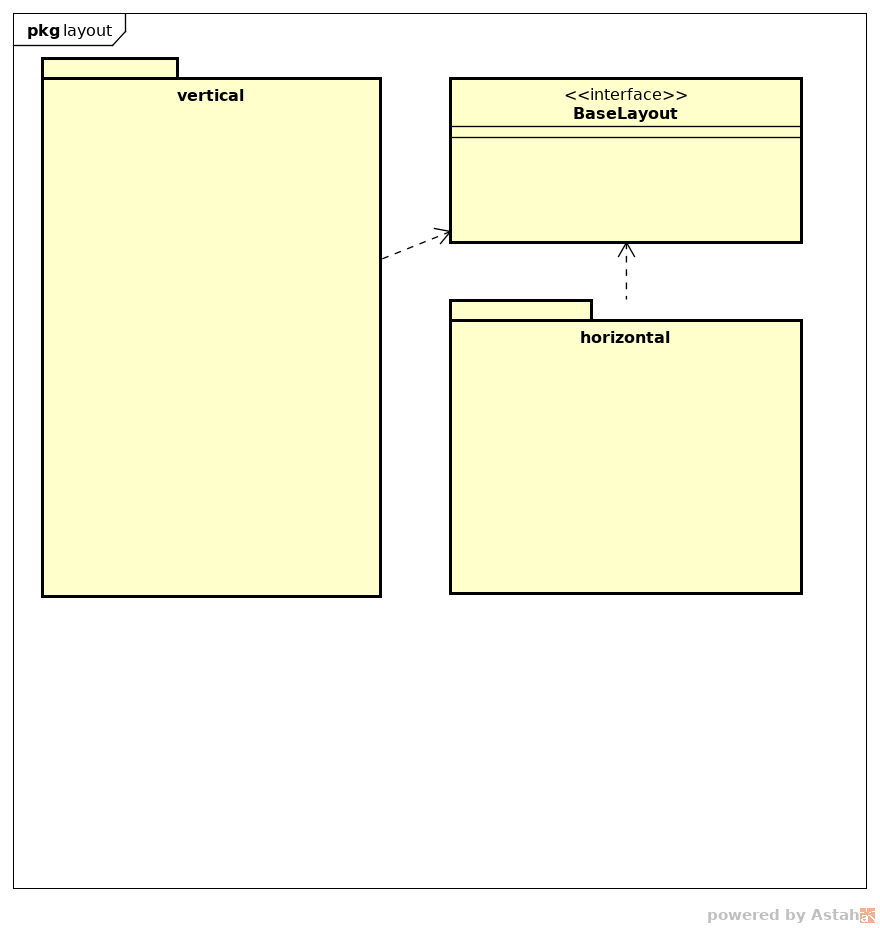
\includegraphics[scale=0.5]{Sezioni/imgPackage/component.png}
	\caption{Monolith::component}
\end{figure}
\begin{itemize}
	\item{\textbf{Descrizione}}: package contenente tutte i packages che permettono la creazione dei componenti di una bolla.
	\item{\textbf{Package e classi contenuti}}:
	\begin{itemize}
	\item{monolith::component::layout}: package contenente tutti i package e classi per la creazione di un \termine{layout}, esso ha la una dipendenza tra i \termine{widget}.
	\item{monolith::component::widget}: package contenente tutti i package per la creazione di un \termine{widget}.
	\item{monolith::component::BaseComponent}: classe interfaccia per un component base.
	\end{itemize}
	
\end{itemize}

\subsubsection{Suddivisione in package  di Monolith::component::layout}
\label{Monolith::component::layout}
\begin{figure}[H]
	\centering
	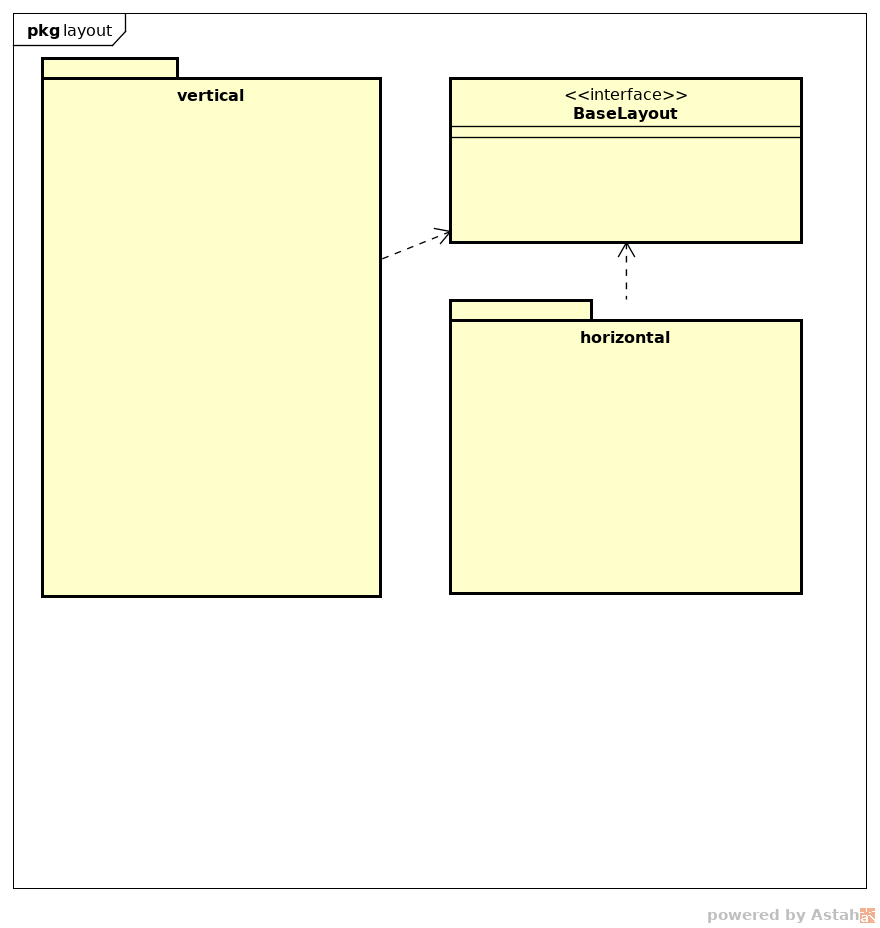
\includegraphics[scale=0.5]{Sezioni/imgPackage/component_layout.png}
	\caption{Monolith::component::layout}
\end{figure}
\begin{itemize}
	\item{\textbf{Descrizione}}: package contenente tutte i packages e classi che permettono la creazione di un layout.
	\item{\textbf{Package e classi contenuti}}:
	\begin{itemize}
	\item{monolith::component::layout::vertical}: package contenente tutti i package e classi per la creazione di un \termine{layout verticale}.
	\item{monolith::component::layout::horizontal}: package contenente tutti i package e classi per la creazione di un \termine{layout orizzontale}.
	\item{monolith::component::layout:BaseLayout}: classe interfaccia per un layout base.
	\end{itemize}
	
\end{itemize}


\subsubsection{Suddivisione in package  di Monolith::component::layout::vertical}
\label{Monolith::component::layout::vertical}
\begin{figure}[H]
	\centering
	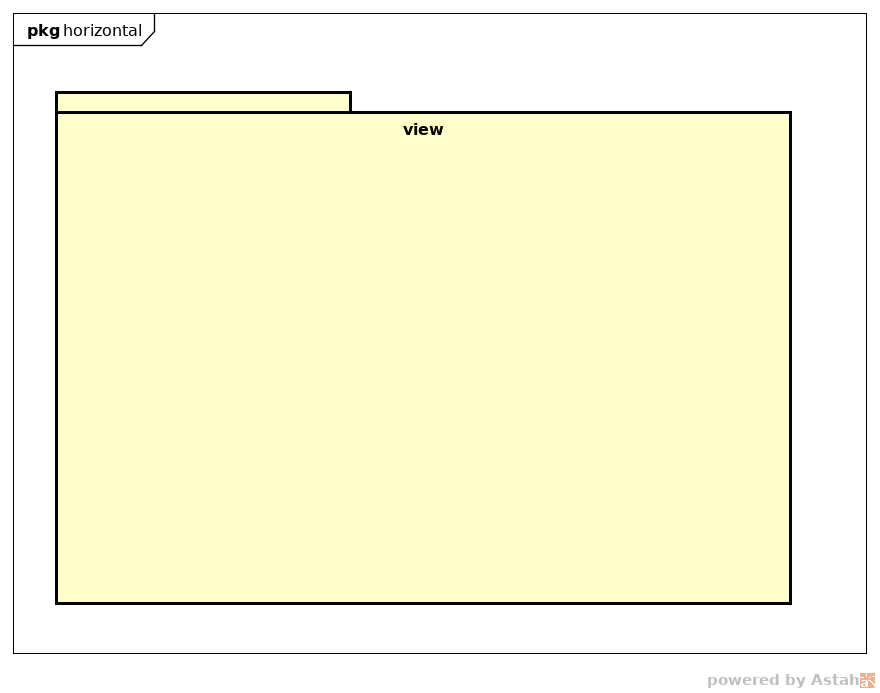
\includegraphics[scale=0.5]{Sezioni/imgPackage/component_layout_vertical.png}
	\caption{Monolith::component::layout::vertical}
\end{figure}
\begin{itemize}
	\item{\textbf{Descrizione}}: package contenente il package view per creare un layout verticale.
	\item{\textbf{Classi contenuti}}:
	\begin{itemize}
	\item{monolith::component::layout::vertical::view}: package contentente la view per la creazione di un layout verticale.
	\end{itemize}
\end{itemize}

\subsubsection{Suddivisione in package  di Monolith::component::layout::horizontal}
\label{Monolith::component::layout::horizontal}
\begin{figure}[H]
	\centering
	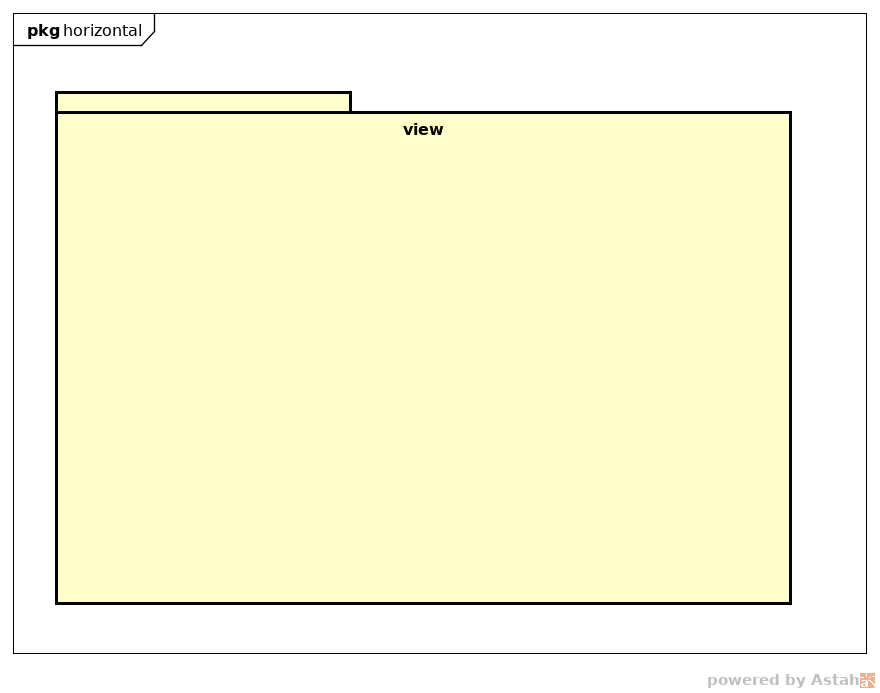
\includegraphics[scale=0.5]{Sezioni/imgPackage/component_layout_horizontal.png}
	\caption{Monolith::component::layout::horizontal}
\end{figure}
\begin{itemize}
	\item{\textbf{Descrizione}}: package contenente il package view per creare un layout orizzontale.
	\item{\textbf{Classi contenuti}}:
	\begin{itemize}
	\item{monolith::component::layout::horizontal::view}: package contentente la view per la creazione di un layout orizzontale.
	\end{itemize}
\end{itemize}

\subsubsection{Suddivisione in package  di Monolith::component::layout::horizontal:view}
\label{Monolith::component::layout::horizontal::view}
\begin{figure}[H]
	\centering
	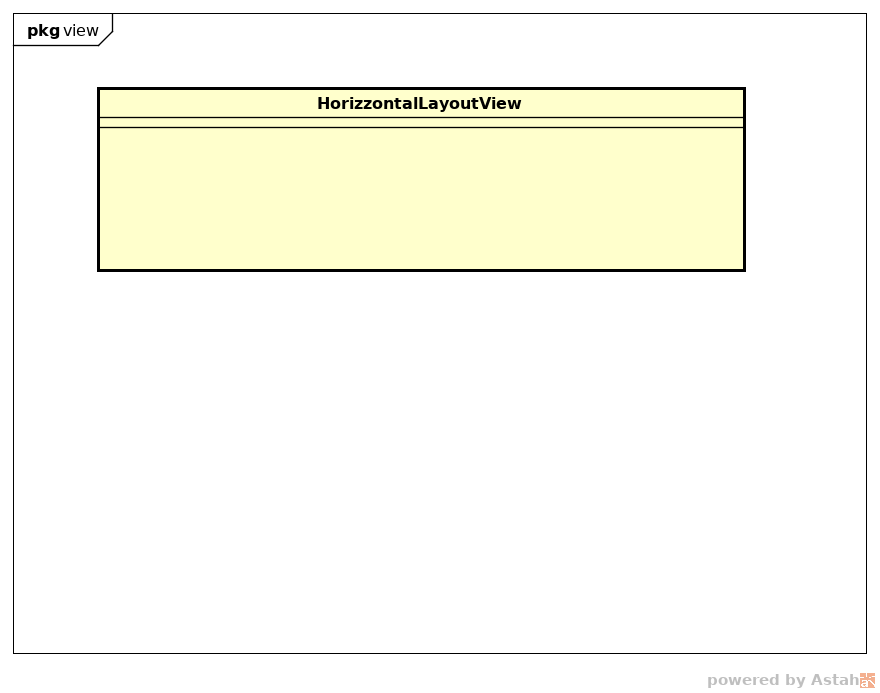
\includegraphics[scale=0.5]{Sezioni/imgPackage/component_layout_horizontal_view.png}
	\caption{Monolith::component::layout::horizontal::view}
\end{figure}
\begin{itemize}
	\item{\textbf{Descrizione}}: package contenente la classe view per creare un layout orizzontale.
	\item{\textbf{Classi contenuti}}:
	\begin{itemize}
	\item{monolith::component::layout::horizontal::view::HorizontalLayoutView}: classe view per la creazione di un layout orizzontale.
	\end{itemize}
\end{itemize}

\subsubsection{Suddivisione in package  di Monolith::component::layout::vertical:view}
\label{Monolith::component::layout::vertical::view}
\begin{figure}[H]
	\centering
	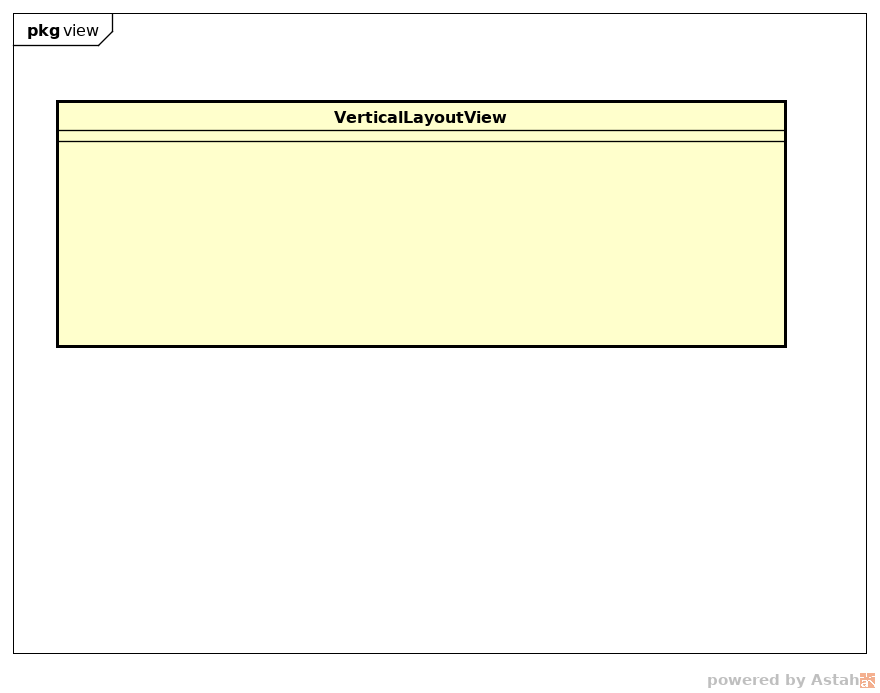
\includegraphics[scale=0.5]{Sezioni/imgPackage/component_layout_vertical_view.png}
	\caption{Monolith::component::layout::vertical::view}
\end{figure}
\begin{itemize}
	\item{\textbf{Descrizione}}: package contenente la classe view per creare un layout verticale.
	\item{\textbf{Classi contenuti}}:
	\begin{itemize}
	\item{monolith::component::layout::vertical::view::VerticalLayoutView}: classe view per la creazione di un layout verticale.
	\end{itemize}
\end{itemize}

\subsubsection{Suddivisione in package  di Monolith::component::widget}
\label{Monolith::component::widget}
\begin{figure}[H]
	\centering
	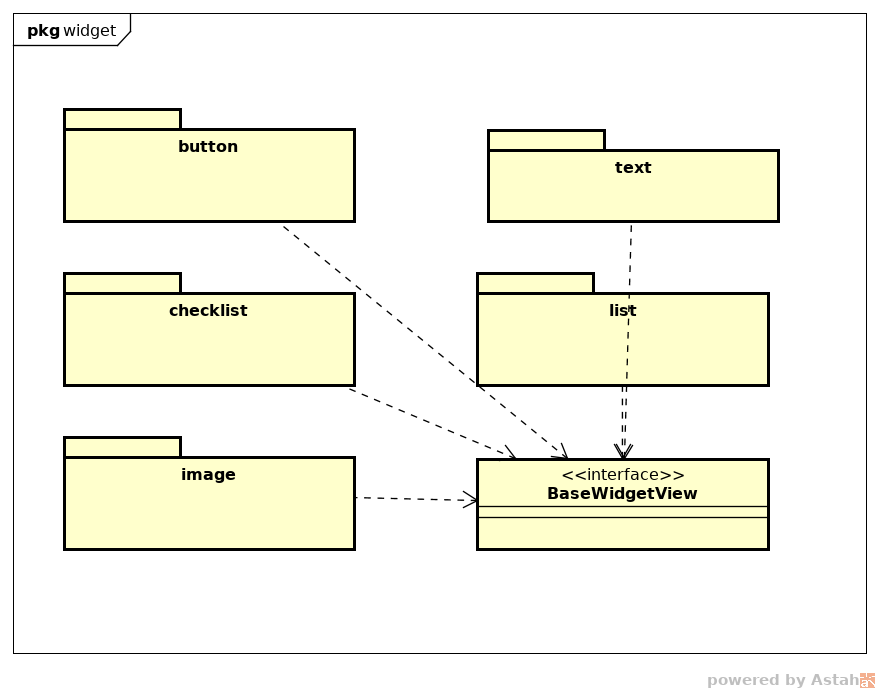
\includegraphics[scale=0.5]{Sezioni/imgPackage/component_widget.png}
	\caption{Monolith::component::widget}
\end{figure}
\begin{itemize}
	\item{\textbf{Descrizione}}: package contenente tutte i packages e classi che permettono la creazione di un \termine{widget}.
	\item{\textbf{Package e classi contenuti}}:
	\begin{itemize}
	\item{monolith::component::widget::button}: package contenente tutti i package e classi per la creazione di un \termine{widget botton}.
	\item{monolith::component::widget::text}: package contenente tutti i package e classi per la creazione di un \termine{widget text}, ha una dipendenza con l'interfaccia BaseWidgetView.
	\item{monolith::component::widget::checklist}: package contenente tutti i package e classi per la creazione di un \termine{widget checklist}, ha una dipendenza con l'interfaccia BaseWidgetView.
	\item{monolith::component::widget::list}: package contenente tutti i package e classi per la creazione di un \termine{widget list}, ha una dipendenza con l'interfaccia BaseWidgetView.
	\item{monolith::component::widget::image}: package contenente tutti i package e classi per la creazione di un \termine{widget image}, ha una dipendenza con l'interfaccia BaseWidgetView.
	\item{monolith::component::widget::BaseWidget}: classe interfaccia per un widget base.
	\end{itemize}
	
\end{itemize}

\subsubsection{Suddivisione in package  di Monolith::component::widget::button}
\label{Monolith::component::widget::button}
\begin{figure}[H]
	\centering
	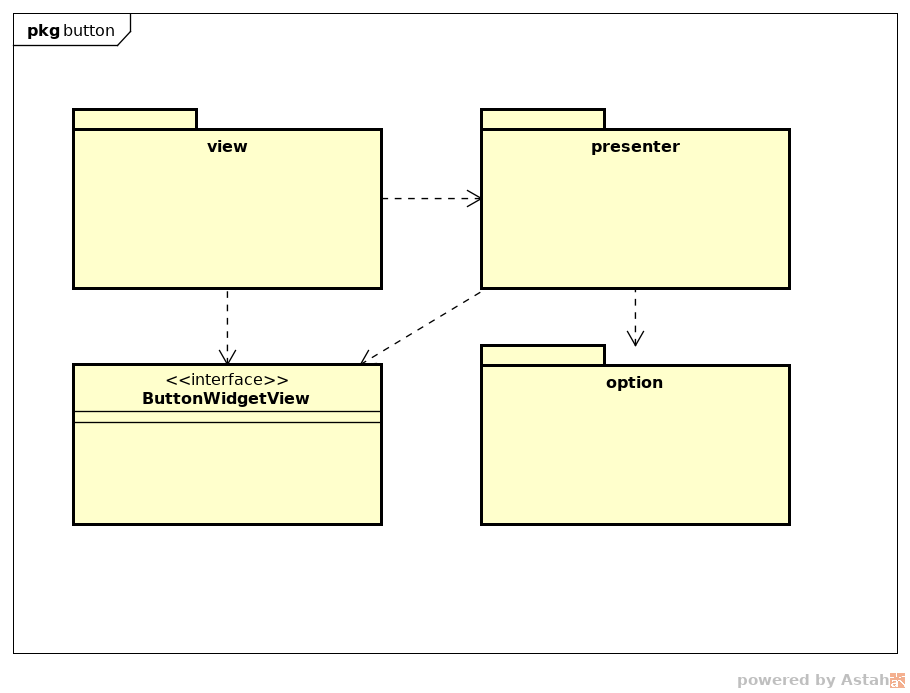
\includegraphics[scale=0.5]{Sezioni/imgPackage/component_widget_button.png}
	\caption{Monolith::component::widget::button}
\end{figure}
\begin{itemize}
	\item{\textbf{Descrizione}}: package contenente tutte i packages e classi che permettono la creazione di un widget button.
	\item{\textbf{Package e classi contenuti}}:
	\begin{itemize}
	\item{monolith::component::widget::button::view}: package contenente tutte le classi per la view di un widget button.
	\item{monolith::component::widget::button::presenter}: package contenente tutte le classi per il presenter di un widget button.
	\item{monolith::component::widget::button::option}: package contenente tutte le classi per le option di un widget button.
	\item{monolith::component::widget::ButtonWidgetView}: classe interfaccia per un widget button.
	\end{itemize}
	
\end{itemize}


\subsubsection{Suddivisione in package  di Monolith::component::widget::button::view}
\label{monolith::component::widget::button::view}
\begin{figure}[H]
	\centering
	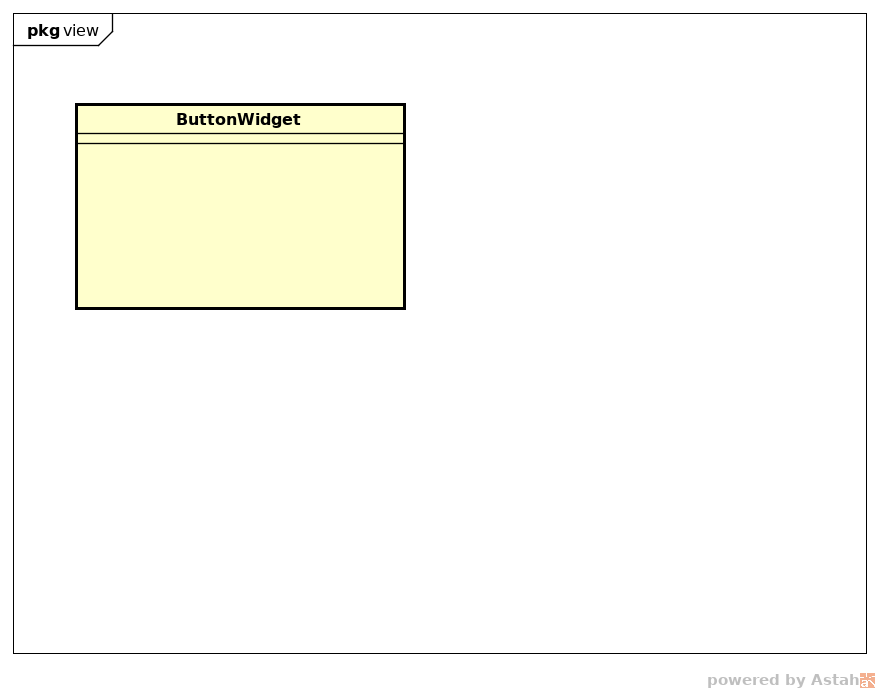
\includegraphics[scale=0.5]{Sezioni/imgPackage/component_widget_button_view.png}
	\caption{monolith::component::widget::button::view}
\end{figure}
\begin{itemize}
	\item{\textbf{Descrizione}}: package contenente la classe view per creare un widget button.
	\item{\textbf{Classi contenuti}}:
	\begin{itemize}
	\item{monolith::component::widget::button::view::ButtonWidget}: classe view per la creazione di un widget button.
	\end{itemize}
\end{itemize}


\subsubsection{Suddivisione in package  di Monolith::component::widget::button::presenter}
\label{monolith::component::widget::button::presenter}
\begin{figure}[H]
	\centering
	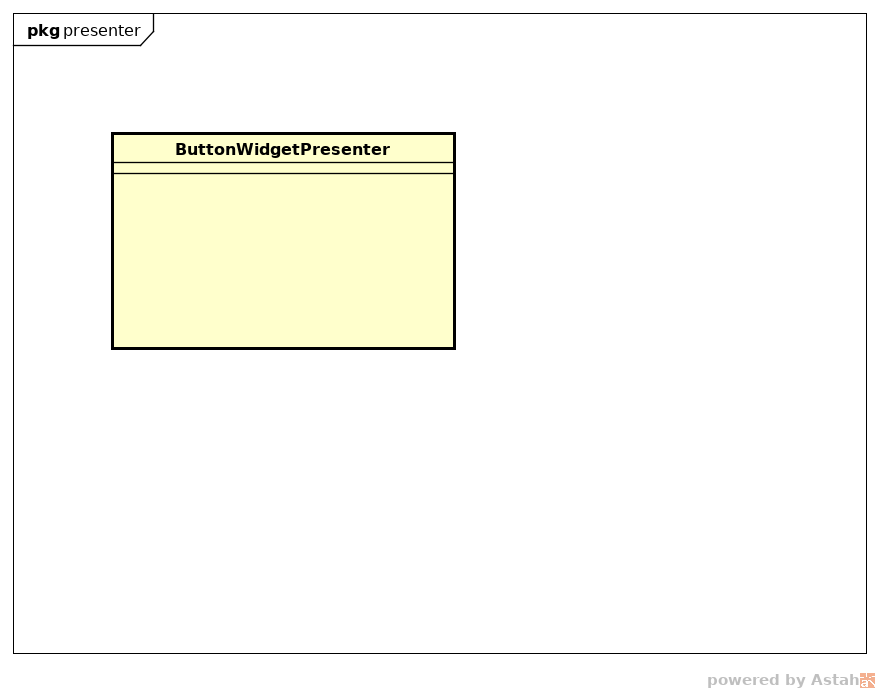
\includegraphics[scale=0.5]{Sezioni/imgPackage/component_widget_button_presenter.png}
	\caption{onolith::component::widget::button::presenter}
\end{figure}
\begin{itemize}
	\item{\textbf{Descrizione}}: package contenente la classe presenter per creare un widget button.
	\item{\textbf{Classi contenuti}}:
	\begin{itemize}
	\item{monolith::component::widget::button::presenter::ButtonWidgetPresenter}: classe presenter per la creazione di un widget button.
	\end{itemize}
\end{itemize}



\subsubsection{Suddivisione in package  di Monolith::component::widget::button::option}
\label{monolith::component::widget::button::option}
\begin{figure}[H]
	\centering
	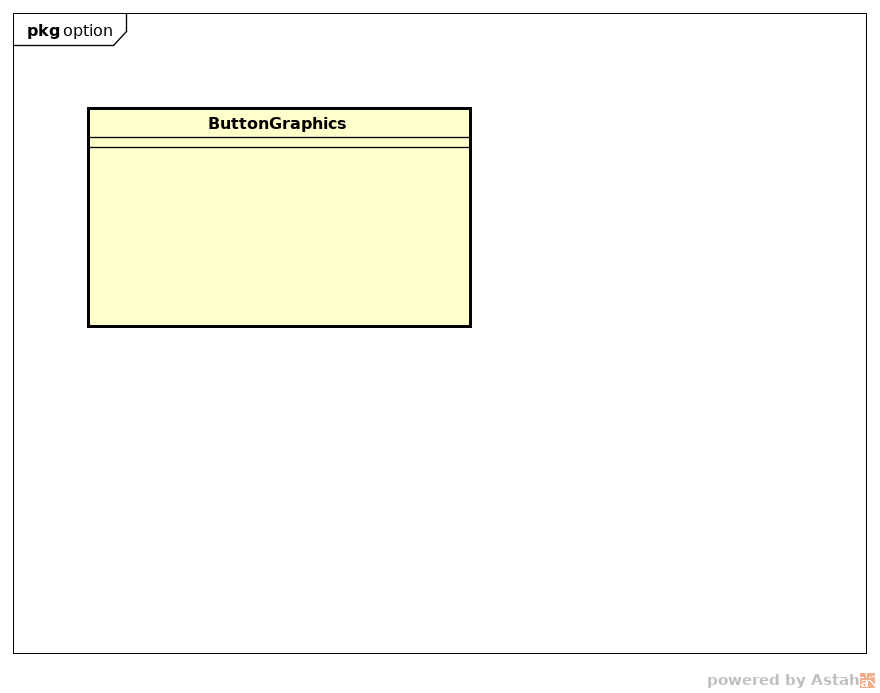
\includegraphics[scale=0.5]{Sezioni/imgPackage/component_widget_button_option.png}
	\caption{monolith::component::widget::button::option}
\end{figure}
\begin{itemize}
	\item{\textbf{Descrizione}}: package contenente la classe option per creare un widget button.
	\item{\textbf{Classi contenuti}}:
	\begin{itemize}
	\item{monolith::component::widget::button::option::ButtonGraphics}: classe per la modifica della grafica di un widget button.
	\end{itemize}
\end{itemize}

\subsubsection{Suddivisione in package  di Monolith::component::widget::checklist}
\label{Monolith::component::widget::checklist}
\begin{figure}[H]
	\centering
	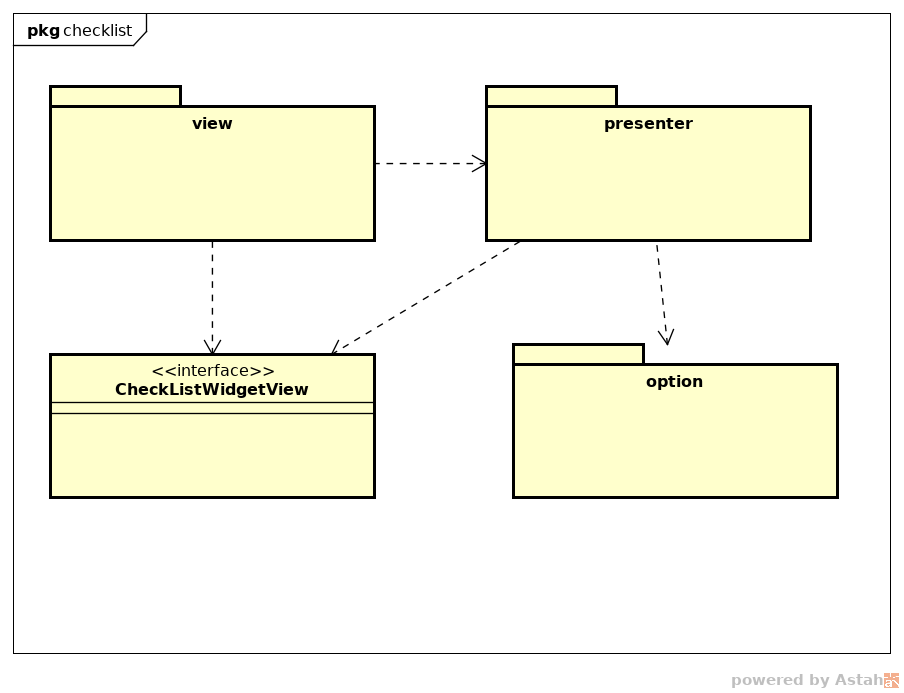
\includegraphics[scale=0.5]{Sezioni/imgPackage/component_widget_checklist.png}
	\caption{Monolith::component::widget::checklist}
\end{figure}
\begin{itemize}
	\item{\textbf{Descrizione}}: package contenente tutte i packages e classi che permettono la creazione di un widget checklist.
	\item{\textbf{Package e classi contenuti}}:
	\begin{itemize}
	\item{monolith::component::widget::checklist::view}: package contenente tutte le classi per la view di un widget checklist.
	\item{monolith::component::widget::checklist::presenter}: package contenente tutte le classi per il presenter di un widget checklist.
	\item{monolith::component::widget::checklist::option}: package contenente tutte le classi per le option di un widget checklist.
	\item{monolith::component::widget::CheckListWidgetView}: classe interfaccia per un widget checklist.
	\end{itemize}
	
\end{itemize}


\subsubsection{Suddivisione in package  di Monolith::component::widget::checklist::view}
\label{monolith::component::widget::checklist::view}
\begin{figure}[H]
	\centering
	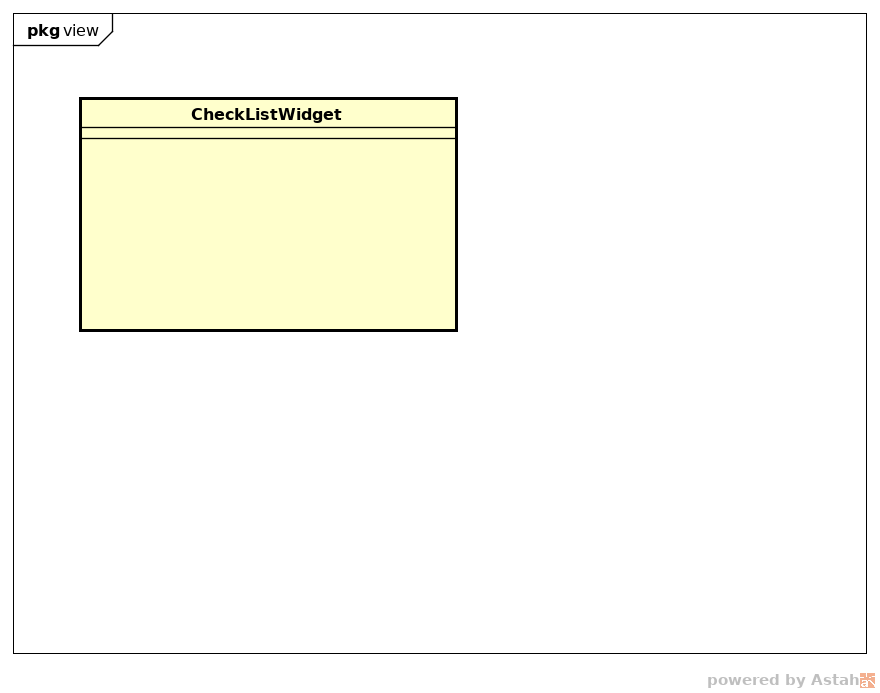
\includegraphics[scale=0.5]{Sezioni/imgPackage/component_widget_checklist_view.png}
	\caption{monolith::component::widget::checklist::view}
\end{figure}
\begin{itemize}
	\item{\textbf{Descrizione}}: package contenente la classe view per creare un widget checklist.
	\item{\textbf{Classi contenuti}}:
	\begin{itemize}
	\item{monolith::component::widget::checklist::view::CheckListWidget}: classe view per la creazione di un widget checklist.
	\end{itemize}
\end{itemize}


\subsubsection{Suddivisione in package  di Monolith::component::widget::checklist::presenter}
\label{monolith::component::widget::checklist::presenter}
\begin{figure}[H]
	\centering
	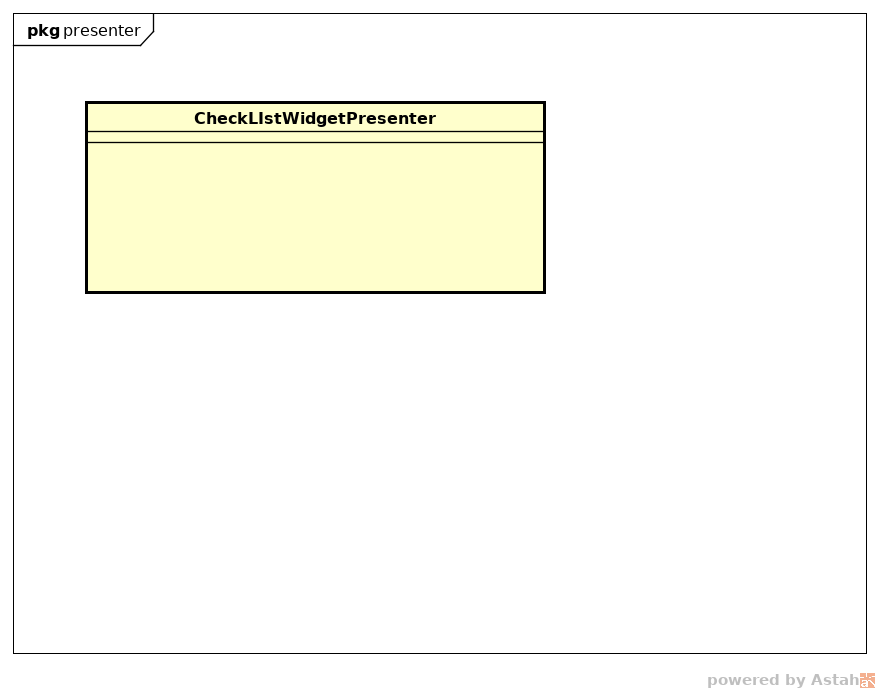
\includegraphics[scale=0.5]{Sezioni/imgPackage/component_widget_checklist_presenter.png}
	\caption{onolith::component::widget::checklist::presenter}
\end{figure}
\begin{itemize}
	\item{\textbf{Descrizione}}: package contenente la classe presenter per creare un widget checklist.
	\item{\textbf{Classi contenuti}}:
	\begin{itemize}
	\item{monolith::component::widget::checklist::presenter::CheckLIstWidgetPresenter}: classe presenter per la creazione di un widget checklist.
	\end{itemize}
\end{itemize}



\subsubsection{Suddivisione in package  di Monolith::component::widget::checklist::option}
\label{monolith::component::widget::checklist::option}
\begin{figure}[H]
	\centering
	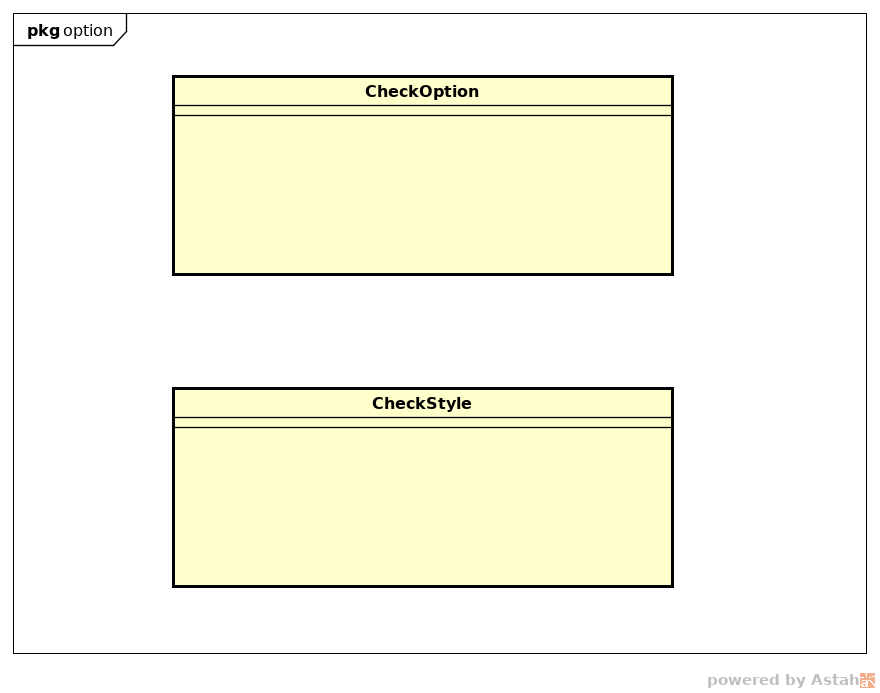
\includegraphics[scale=0.5]{Sezioni/imgPackage/component_widget_checklist_option.png}
	\caption{onolith::component::widget::checklist::option}
\end{figure}
\begin{itemize}
	\item{\textbf{Descrizione}}: package contenente le classi option per creare un widget checklist.
	\item{\textbf{Classi contenuti}}:
	\begin{itemize}
	\item{monolith::component::widget::checklist::option::CheckOption}: classe per la modifica della proprietà di spunta del widget checklist.
	\item{monolith::component::widget::checklist::option::CheckStyle}: classe per la modifica della grafica di spunta del widget checklist.
	\end{itemize}
\end{itemize}


\subsubsection{Suddivisione in package  di Monolith::component::widget::image}
\label{Monolith::component::widget::image}
\begin{figure}[H]
	\centering
	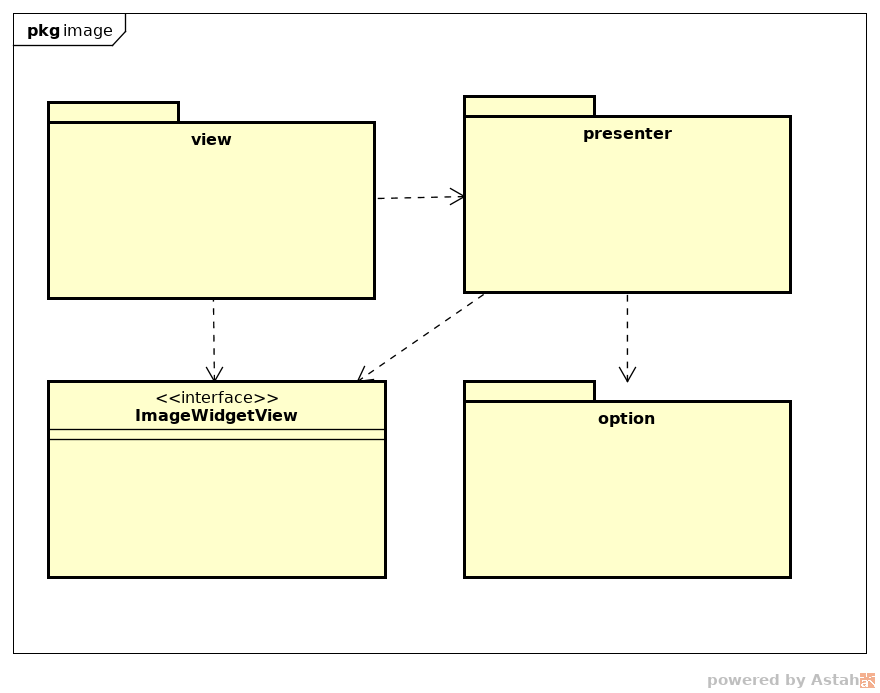
\includegraphics[scale=0.5]{Sezioni/imgPackage/component_widget_image.png}
	\caption{Monolith::component::widget::image}
\end{figure}
\begin{itemize}
	\item{\textbf{Descrizione}}: package contenente tutte i packages e classi che permettono la creazione di un widget image.
	\item{\textbf{Package e classi contenuti}}:
	\begin{itemize}
	\item{monolith::component::widget::image::view}: package contenente tutte le classi per la view di un widget image.
	\item{monolith::component::widget::image::presenter}: package contenente tutte le classi per il presenter di un widget image.
	\item{monolith::component::widget::image::option}: package contenente tutte le classi per le option di un widget image.
	\item{monolith::component::widget::image:ImageWidgetView}: classe interfaccia per un widget image.
	\end{itemize}
	
\end{itemize}


\subsubsection{Suddivisione in package  di Monolith::component::widget::image::view}
\label{monolith::component::widget::image::view}
\begin{figure}[H]
	\centering
	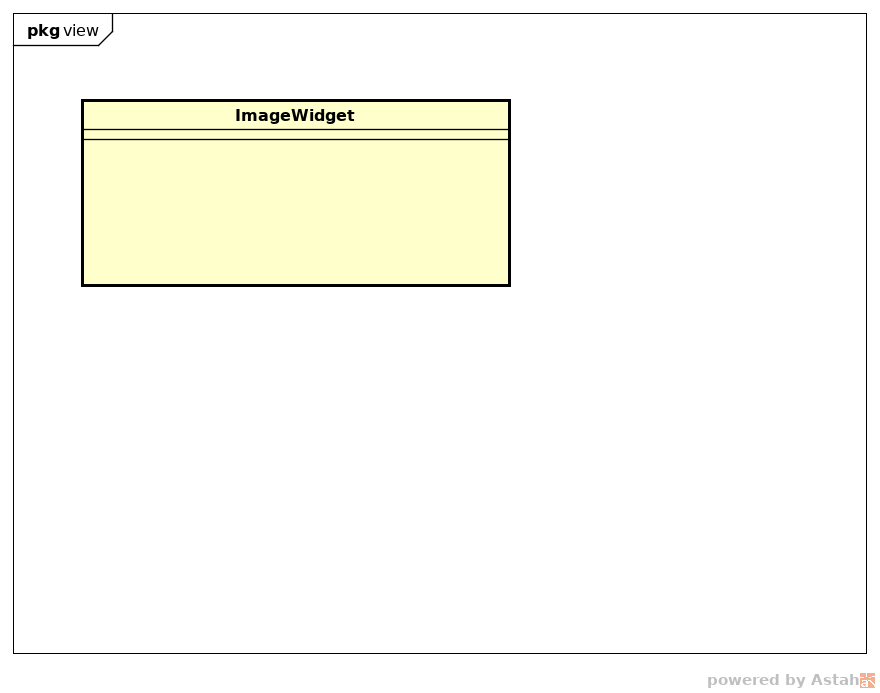
\includegraphics[scale=0.5]{Sezioni/imgPackage/component_widget_image_view.png}
	\caption{monolith::component::widget::image::view}
\end{figure}
\begin{itemize}
	\item{\textbf{Descrizione}}: package contenente la classe view per creare un widget image.
	\item{\textbf{Classi contenuti}}:
	\begin{itemize}
	\item{monolith::component::widget::checklist::view::ImageWidget}: classe view per la creazione di un widget image.
	\end{itemize}
\end{itemize}


\subsubsection{Suddivisione in package  di Monolith::component::widget::image::presenter}
\label{monolith::component::widget::image::presenter}
\begin{figure}[H]
	\centering
	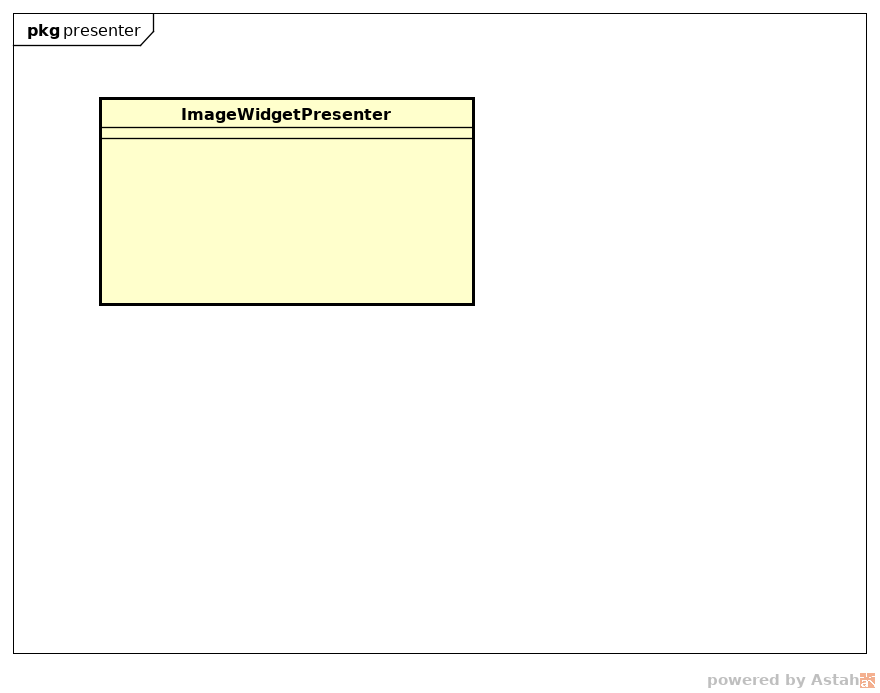
\includegraphics[scale=0.5]{Sezioni/imgPackage/component_widget_image_presenter.png}
	\caption{monolith::component::widget::image::presenter}
\end{figure}
\begin{itemize}
	\item{\textbf{Descrizione}}: package contenente la classe presenter per creare un widget image.
	\item{\textbf{Classi contenuti}}:
	\begin{itemize}
	\item{monolith::component::widget::checklist::image::ImageWidgetPresenter}: classe presenter per la creazione di un widget image.
	\end{itemize}
\end{itemize}



\subsubsection{Suddivisione in package  di Monolith::component::widget::image::option}
\label{onolith::component::widget::image::option}
\begin{figure}[H]
	\centering
	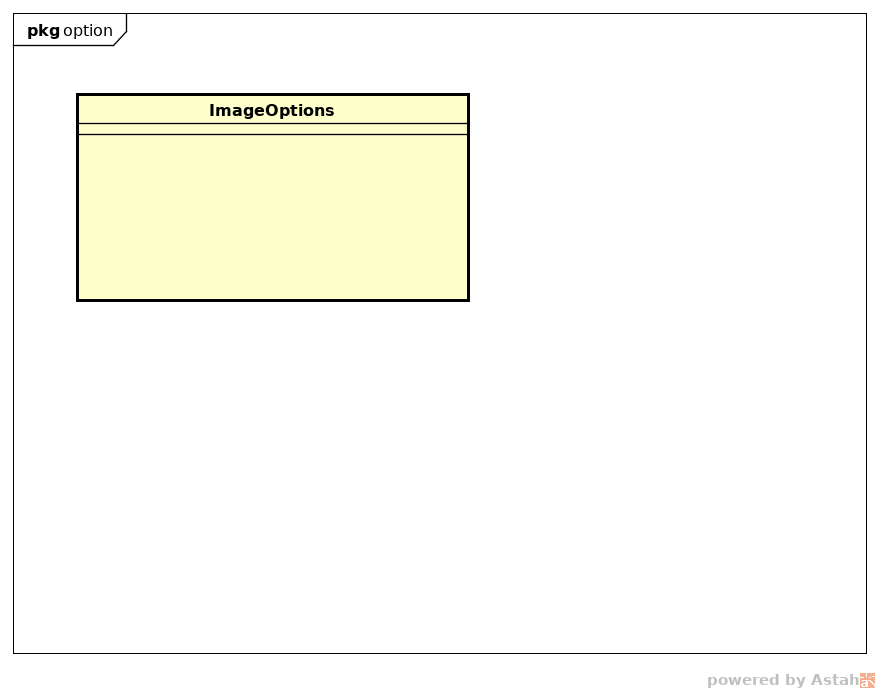
\includegraphics[scale=0.5]{Sezioni/imgPackage/component_widget_image_option.png}
	\caption{onolith::component::widget::image::option}
\end{figure}
\begin{itemize}
	\item{\textbf{Descrizione}}: package contenente le classi option per creare un widget image.
	\item{\textbf{Classi contenuti}}:
	\begin{itemize}
	\item{monolith::component::widget::image::option::ImageOptions}: classe per la modifica della proprietà dell'immagine del widget image.
	\end{itemize}
\end{itemize}


\subsubsection{Suddivisione in package  di Monolith::component::widget::list}
\label{Monolith::component::widget::list}
\begin{figure}[H]
	\centering
	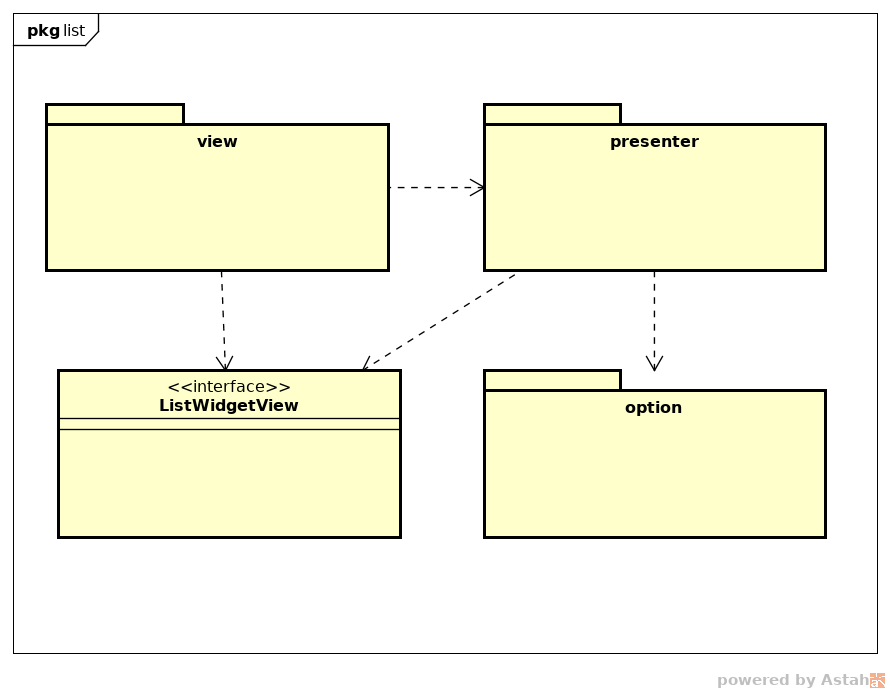
\includegraphics[scale=0.5]{Sezioni/imgPackage/component_widget_list.png}
	\caption{Monolith::component::widget::list}
\end{figure}
\begin{itemize}
	\item{\textbf{Descrizione}}: package contenente tutte i packages e classi che permettono la creazione di un widget list.
	\item{\textbf{Package e classi contenuti}}:
	\begin{itemize}
	\item{monolith::component::widget::list::view}: package contenente tutte le classi per la view di un widget list.
	\item{monolith::component::widget::list::presenter}: package contenente tutte le classi per il presenter di un widget list.
	\item{monolith::component::widget::list::option}: package contenente tutte le classi per le option di un widget list.
	\item{monolith::component::widget::list:ListWidgetView}: classe interfaccia per un widget .
	\end{itemize}
	
\end{itemize}


\subsubsection{Suddivisione in package  di Monolith::component::widget::list::view}
\label{monolith::component::widget::list::view}
\begin{figure}[H]
	\centering
	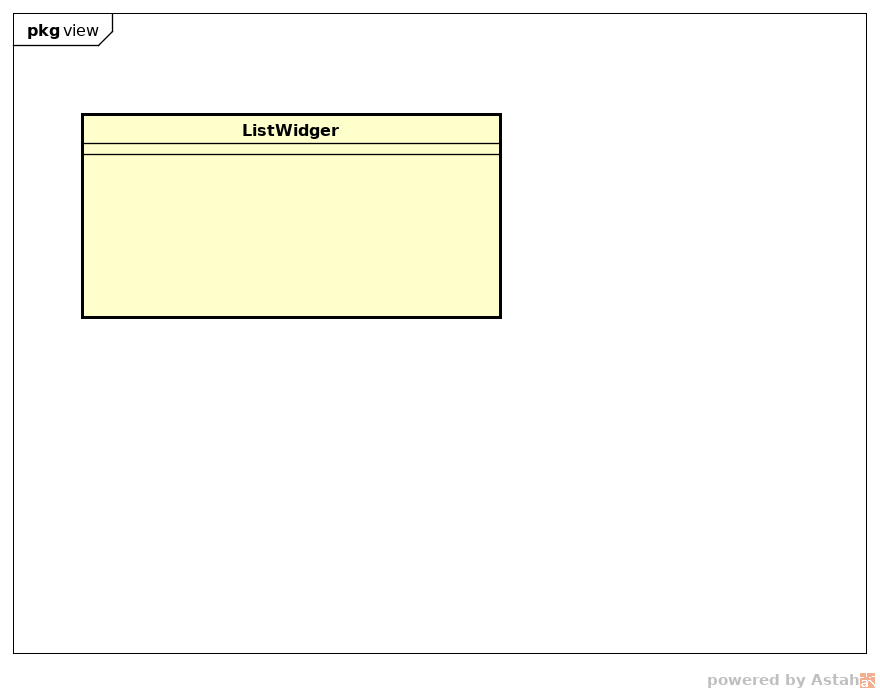
\includegraphics[scale=0.5]{Sezioni/imgPackage/component_widget_list_view.png}
	\caption{monolith::component::widget::list::view}
\end{figure}
\begin{itemize}
	\item{\textbf{Descrizione}}: package contenente la classe view per creare un widget list.
	\item{\textbf{Classi contenuti}}:
	\begin{itemize}
	\item{monolith::component::widget::list::view::ListWidger}: classe view per la creazione di un widget image.
	\end{itemize}
\end{itemize}


\subsubsection{Suddivisione in package  di Monolith::component::widget::list::presenter}
\label{monolith::component::widget::list::presenter}
\begin{figure}[H]
	\centering
	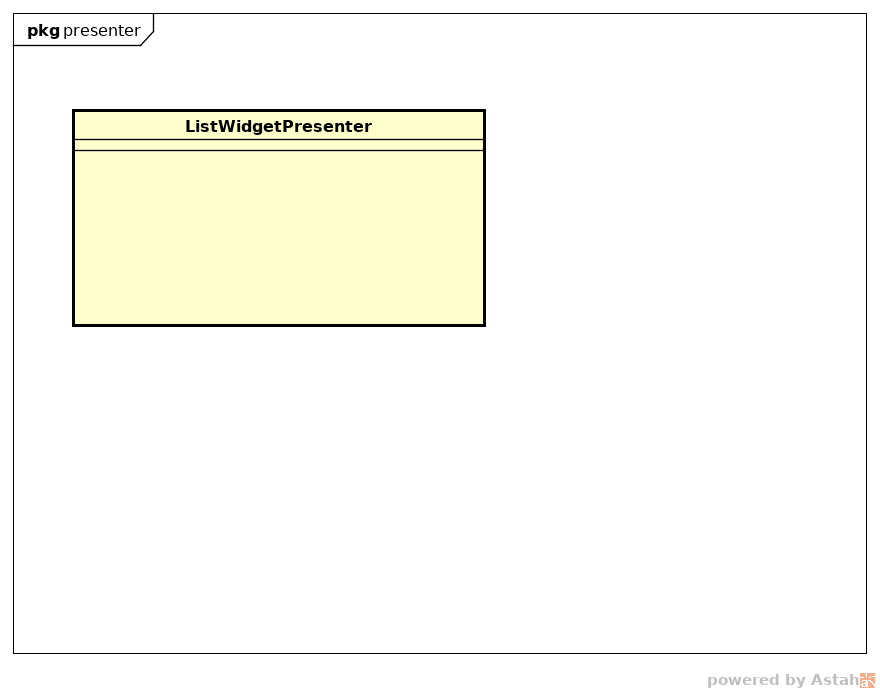
\includegraphics[scale=0.5]{Sezioni/imgPackage/component_widget_list_presenter.png}
	\caption{monolith::component::widget::list::presenter}
\end{figure}
\begin{itemize}
	\item{\textbf{Descrizione}}: package contenente la classe presenter per creare un widget list.
	\item{\textbf{Classi contenuti}}:
	\begin{itemize}
	\item{monolith::component::widget::list::image::ListWidgetPresenter}: classe presenter per la creazione di un widget list.
	\end{itemize}
\end{itemize}



\subsubsection{Suddivisione in package  di Monolith::component::widget::list::option}
\label{monolith::component::widget::list::option}
\begin{figure}[H]
	\centering
	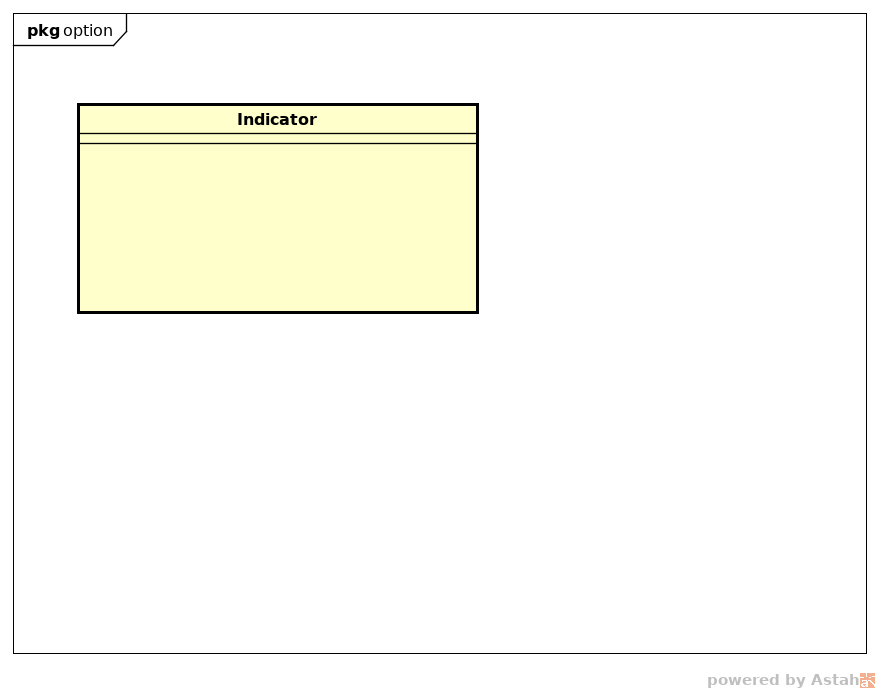
\includegraphics[scale=0.5]{Sezioni/imgPackage/component_widget_list_option.png}
	\caption{onolith::component::widget::list::option}
\end{figure}
\begin{itemize}
	\item{\textbf{Descrizione}}: package contenente le classi option per creare un widget list.
	\item{\textbf{Classi contenuti}}:
	\begin{itemize}
	\item{monolith::component::widget::list::option::Indicator}: classe per la modifica della proprietà dell'indicatore del singolo item del widget list.
	\end{itemize}
\end{itemize}




\subsubsection{Suddivisione in package  di Monolith::component::widget::text}
\label{Monolith::component::widget::text}
\begin{figure}[H]
	\centering
	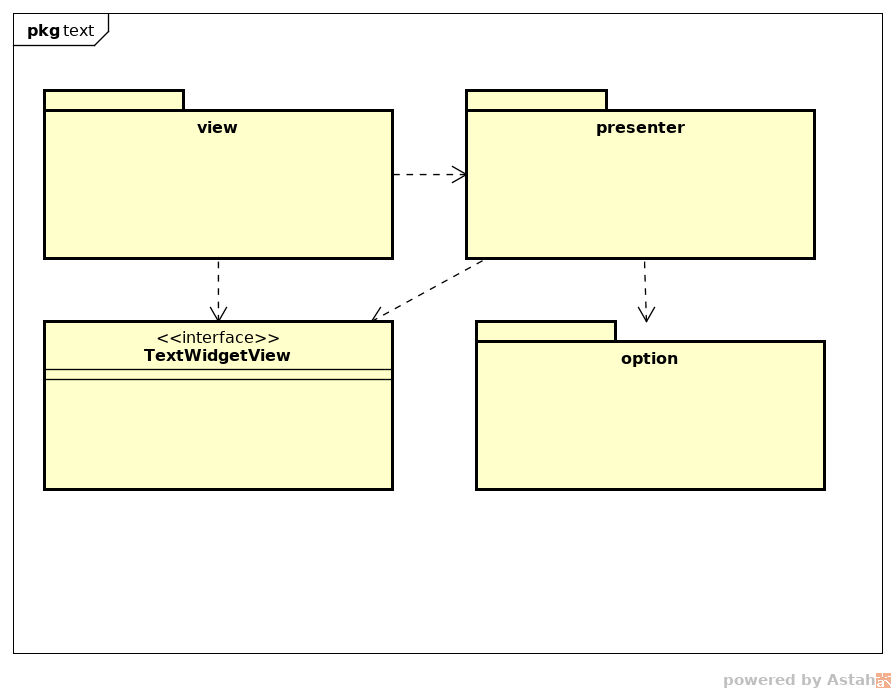
\includegraphics[scale=0.5]{Sezioni/imgPackage/component_widget_text.png}
	\caption{Monolith::component::widget::text}
\end{figure}
\begin{itemize}
	\item{\textbf{Descrizione}}: package contenente tutte i packages e classi che permettono la creazione di un widget text.
	\item{\textbf{Package e classi contenuti}}:
	\begin{itemize}
	\item{monolith::component::widget::text::view}: package contenente tutte le classi per la view di un widget text.
	\item{monolith::component::widget::text::presenter}: package contenente tutte le classi per il presenter di un widget text.
	\item{monolith::component::widget::text::option}: package contenente tutte le classi per le option di un widget text.
	\item{monolith::component::widget::text:TextWidgetView}: classe interfaccia per un widget text.
	\end{itemize}
	
\end{itemize}


\subsubsection{Suddivisione in package  di Monolith::component::widget::text::view}
\label{monolith::component::widget::text::view}
\begin{figure}[H]
	\centering
	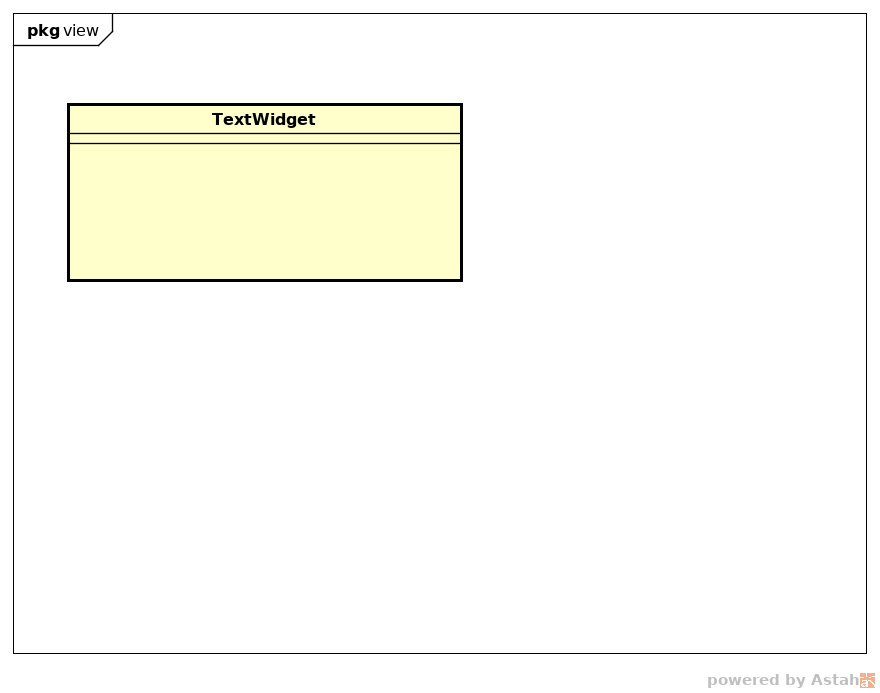
\includegraphics[scale=0.5]{Sezioni/imgPackage/component_widget_text_view.png}
	\caption{monolith::component::widget::text::view}
\end{figure}
\begin{itemize}
	\item{\textbf{Descrizione}}: package contenente la classe view per creare un widget text.
	\item{\textbf{Classi contenuti}}:
	\begin{itemize}
	\item{monolith::component::widget::text::view::TextWidget}: classe view per la creazione di un widget text.
	\end{itemize}
\end{itemize}


\subsubsection{Suddivisione in package  di Monolith::component::widget::text::presenter}
\label{monolith::component::widget::text::presenter}
\begin{figure}[H]
	\centering
	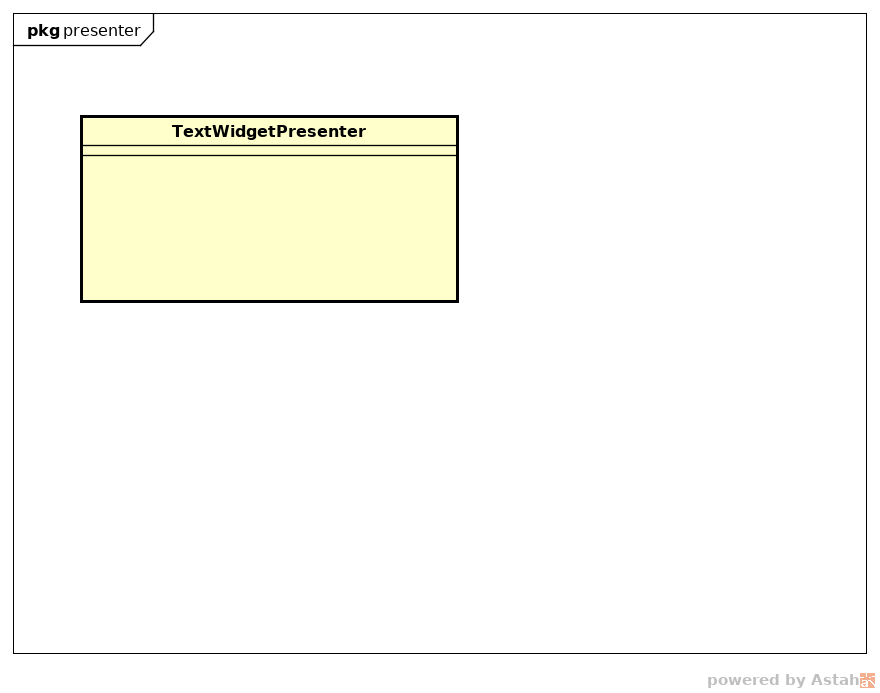
\includegraphics[scale=0.5]{Sezioni/imgPackage/component_widget_text_presenter.png}
	\caption{monolith::component::widget::text::presenter}
\end{figure}
\begin{itemize}
	\item{\textbf{Descrizione}}: package contenente la classe presenter per creare un widget text.
	\item{\textbf{Classi contenuti}}:
	\begin{itemize}
	\item{monolith::component::widget::text::TextWidgetPresenter}: classe presenter per la creazione di un widget text.
	\end{itemize}
\end{itemize}



\subsubsection{Suddivisione in package  di Monolith::component::widget::text::option}
\label{monolith::component::widget::text::option}
\begin{figure}[H]
	\centering
	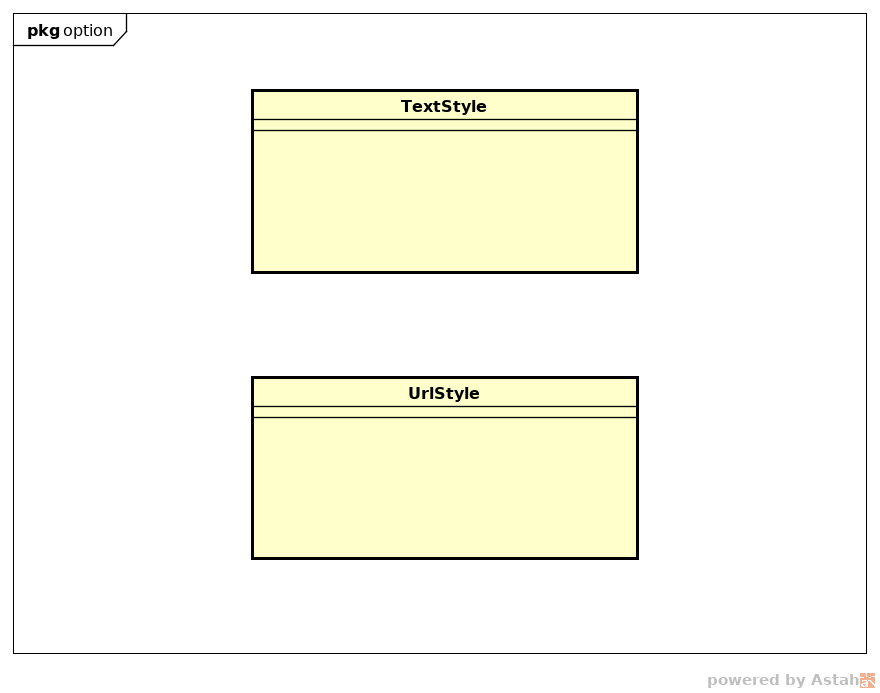
\includegraphics[scale=0.5]{Sezioni/imgPackage/component_widget_text_option.png}
	\caption{onolith::component::widget::text::option}
\end{figure}
\begin{itemize}
	\item{\textbf{Descrizione}}: package contenente le classi option per creare un widget text.
	\item{\textbf{Classi contenuti}}:
	\begin{itemize}
	\item{monolith::component::widget::text::option::TextStyle}: classe per la modifica dello stile di testo del widget text.
	\item{monolith::component::widget::text::option::UrlStyle}: classe per la modifica dello stile dell' url del widget text.
	\end{itemize}
\end{itemize}






\newpage